%only here
DM produced at colliders would register just as neutrinos do, which is to say: not at all. 
In this chapter, we describe DM production from a pragmatic, collider physicist's perspective, focusing on a selection of simple models with distinct and testable LHC signatures\footnote{For other perspectives, see Refs.~\cite{Kahlhoefer:2017dnp,Abercrombie:2015wmb,Arcadi:2017kky,Feng:2010gw}.}.
Moreover, we will use the term {\it invisible particles} (\IP) rather than DM when emphasizing that detecting such particles need not be a discovery of DM\footnote{For example, invisible particles may decay after leaving the detector, a decay that is essential prompt on cosmological time scales.}.

%%% what we have in chapter 2

The body of DM model literature can be divided into two extremes.%, each driving experimental searches in two complementary directions.
Fully-realized, self-consistent models such as SUSY provide specific features that can be exploited for narrowly-targeted searches, while simplified models with a few ingredients can capture broad collider signatures of classes of models, serving as benchmarks for more general but less optimal searches.
Key to both are the determinative details of the interactions between the DM and the SM, rather than the DM itself.



%These models will be described in the next section.
%sentence cut from here
%The success of such simple, at times incomplete and not always theoretically sound models has been due to their ability to predict the key features and observables related to DM production at the LHC with only a limited number of new particles and theory parameters, factoring out the more complex processes that do not affect LHC phenomenology as they e.g. occur at higher energy scales. As proven by the history of SM discoveries, this simple approach can be used to discover the most prominent DM-SM interaction processes in the wake of the LHC start-up. 

To restrict the scope of this review,
%% -To narrow our choice of DM models to those  assumptions to

%% to models that are more widely studied:


\begin{enumerate}
\item we describe only models where the DM interacts with SM hadrons, either directly or effectively;
\item we privilege models that include a $Z_2$ symmetry to stabilize DM;
\item we emphasize models connecting to a thermal, frozen-out relic; others, based on alternate cosmological histories (e.g. freeze-in), also have interesting LHC signatures~\cite{Bernal:2017kxu}

%Citation from DMFs
%[49] J. Abdallah, H. Araujo, A. Arbey, A. Ashkenazi, A. Belyaev, et al., Simplified models for dark matter searches at the LHCSubmitted to Phys.Dark Univ. arXiv:1506.03116.
% [47] A. A. Petrov, W. Shepherd, Searching for dark matter at LHC with mono- Higgs production, Phys.Lett. B730 (2014) 178–183. arXiv:1311.1511, doi:10.1016/j.physletb.2014.01.051.
% [51] R. S. Chivukula, H. Georgi, Composite Technicolor Standard Model, Phys.Lett. B188 (1987) 99. doi:10.1016/0370-2693(87)90713-1.
% [52] L. Hall, L. Randall, Weak scale effective supersymmetry, Phys.Rev.Lett. 65 (1990) 2939–2942. doi:10.1103/PhysRevLett.65.2939.
% 2570 [53]
% A. Buras, P. Gambino, M. Gorbahn, S. Jager, L. Silvestrini, Universal unitarity triangle and physics beyond the Standard Model, Phys.Lett. B500 (2001) 161–167. arXiv:hep-ph/0007085, doi:10.1016/S0370-2693(01) 00061-2.
% 2575
% [54] G. D’Ambrosio, G. Giudice, G. Isidori, A. Strumia, Minimal Flavor Viola- tion: An effective field theory approach, Nucl.Phys. B645 (2002) 155–187. arXiv:hep-ph/0207036, doi:10.1016/S0550-3213(02)00836-2.
\item we stress models employed for early LHC Run-2 searches, where the DM is a Dirac fermion, and the model mimics the pattern of flavor violation found in the SM (Minimal Flavor Violation, or MFV~\cite{DAmbrosio:2002vsn}).
%Other cases yield similar phenomenology for LHC searches, with some exceptions that we describe in this chapter.
%The Dawn of FIMP Dark Matter: A Review of Models and Constraints  - https://arxiv.org/pdf/1706.07442.pdf, Minimal Decaying Dark Matter and the LHC - https://arxiv.org/pdf/1305.6587.pdf
\end{enumerate}
Departures from these assumptions are discussed further in~\cite{Abercrombie:2015wmb}. 

%In the following we enumerate the possible reactions of DM at colliders within these assumptions.

\subsection{Higgs and Z boson portals}
\label{sec:HZPortalModels}

%Simple models connecting DM to SM through the bosons of the SM 

Extending the SM with a single DM particle, and nothing else, one may arrive at portal models where the Z or Higgs boson mediates the DM--SM interaction.%, which economically relate DM to the SM fermions through a neutral gauge boson.
This is our first example of a {\it mediator}, a 'dark sector' particle that governs the DM-SM interaction.
While the \textbf{Z portal} is perhaps the simplest model of DM that one can construct, LEP and direct detection experiments strongly constrain it, as discussed in Sec.~\ref{sec:results_ZHSearches}. 
\textbf{Higgs portal} models~\cite{Patt:2006fw,Englert:2011yb,Djouadi:2011aa} are more promising, as only the recent generations of collider and direct detection experiments has reached the energies and luminosities necessary to search for them.%faintly-coupled mediators with EW-scale (Higgs-scale) masses.
Direct collider searches for the invisibly-decaying Higgs bosons are augmented by measurements of other Higgs properties, which can be very sensitive to couplings to new particles.

The Z and Higgs portal models have relatively simple phenomenology.
The mediators (the Z or Higgs boson) are light in comparison to the LHC energy and can be produced on-shell.
Even if the \IP are much heavier, and invisible decays of the mediator are absent, collider searches may still study the Z and Higgs and constrain these models through their fully-visible decays.

%% For scalar or vector DM, this interaction is renormalizable and leads to a UV-complete theory. If DM is a fermion, further particles mediating the interaction are required to make the theory self-consistent~\cite{Freitas:2015hsa,Escudero:2016gzx,deSimone:2014pda}. 
%% For fermionic DM heavier than a few TeV, the model is not perturbative anymore. 

% No other SM particle can serve as portal at leading order.  
%We start from models that do not add any other particle to the SM except the DM and later continue to models with more complex particle content and interactions. 

%% Models where the SM particle sector is coupled to DM through an existing or a new particle are called \textit{portal models}.
%% Models where the SM particle sector is coupled to the dark sector through an existing or a new particle are called portal models.

%If one adds only a neutral DM particle to the SM content, one arrives at 

%Models where the SM particle sector is coupled to the dark sector through an existing or a new particle are called \textit{portal models}. This kind of model leads to the most economical particle content for reactions at the LHC, as one only needs to add a neutral DM particle to the SM content if one of the SM particles is the portal particle. SM fermions cannot be portal particles under the assumption of a $Z_2$ symmetry, as they would allow the decay of DM. Photons, W bosons and gluons can't be portal particles either, as DM does not absorb nor emit light, nor it does it have electromagnetic or strong charge. The only viable SM portal particles remaining are the Z and the Higgs bosons.


%% These

%% It is natural to have mediators at this scale within DM theories predicting new weakly interacting particles~\cite{Cotta:2012nj,Arcadi:2014lta}.
%% However, only the recent generations of collider and direct detection experiments have had sufficient energy and luminosity to search for faintly-coupled mediators with EW-scale (Higgs-scale) masses.


%% There are compelling theoretical and experimental arguments for these models
%% The electroweak (EW) scale seems to be a special energy scale in nature, where the weak bosons, Higgs boson, and top quark masses lay.



%% The discovery of a SM-like Higgs boson
%~\cite{Aad:2012tfa,Chatrchyan:2012xdj} 
%% has now made it possible to test 
%and references therein? In case there is more room for H portal citations, should cite also: 
%https://arxiv.org/pdf/1304.2417.pdf
%From Escudero:2016gzx
%We point out that for fermionic dark matter heavier than several TeV, perturbative unitarity is lost, and higher dimension operators such as those ones considered in ref. [10] may become relevant for the phenomenology. It is interesting to note that within the context of the MSSM, a bino-like neutralino (with a subdominant higgsino fraction) can possess the characteristics found within this scenario [11].
%The couplings of the Higgs to DM can be scalar or pseudoscalar. This may need to be discussed later. 
%Another completion of the Dirac DM:
%S. Baek, P. Ko, and W.-I. Park, Search for the Higgs portal to a singlet fermionic dark matter at the LHC, J. High Energy Phys. 1202 047, (2012), [arXiv:1112.1847].
%From http://iopscience.iop.org/article/10.1088/1126-6708/2008/07/058/pdf
%Higgs-sector and Z′ interactions between the hidden sector
%and the SM states are special in that they involve gauge-invariant operators of dimension
%dO ≤ 4, and thus can be induced by physics at arbitrarily high scales with unsuppressed
%couplings. 
%This class of models is already constrained by electroweak precision measurements, but still viable if the DM mass is about half the Higgs mass. 

%We could have a picture of constraints here?

%Arcadi
%However, the last LUX results[11], combined with the invisi- ble width of the Higgs excluded the Higgs-portal scenario for dark matter mass below 200 GeV [2].

\subsection{Effective Field Theories and Simplified models of BSM mediators}
\label{sec:BSMMediatorModels}

One step further in complexity beyond the Z and Higgs portal models are models where the mediator is also a new particle, such as a heavier version of the $Z$ boson (a $Z^\prime$) or an additional scalar.

%If the new mediators are light enough for the LHC to produce them on-shell, one can observe them via their invisible decays and also via their resonant decays to SM.
%If, on the other hand, the mediator is a relatively heavy BSM particle, a situation arises similar to the Fermi model of weak interactions.



%~\cite{Fermi2008}. 

%The adoption of much simpler model as first LHC Run-2 DM benchmarks led to the design of more generic searches targeting the broad features of those models. 

\subsubsection{Effective Field Theories}
\label{sub:EFT}

%Colliders cannot detect neutrinos directly but can detect particles coupled to the W and Z bosons, the nature of which are determined by the details of the weak interaction.
%Since the nature of the interaction between SM and DM remains a mystery, we do not know these determinative details.

In some situations, such as when a BSM mediator is heavy compared to the collision energy, the DM--SM interaction appears to be a contact interaction, with all observables completely determined by one rate parameter, the contact interacion scale, that controls the production rate, and a Lorentz structure choice, which has a modest effect on the transverse momentum distributions of the invisible particles.
In this case, Effective Field Theories (EFTs)~\cite{Goodman:2010ku, Shoemaker:2011vi,Bai:2010hh} provide a description of the production of invisible particles.
A sketch of an EFT process is shown in panel (a) of Fig.~\ref{fig:monoX}.
One may hope that such as description is sufficient for the LHC; the unknown high-energy details of a complicated interaction are conveniently integrated out.
Moreover, since EFTs do not fix a mediation mechanism, they provide a framework to systematically explore a wide range of possible physics.

%For example, in the case of a $s-$channel completion of the EFT, this interaction scale is proportional to the mass of the mediator particle, which is in turn related to the momentum transfer. 

If, instead, the interaction physics is kinematically accessible (e.g., the mediator mass is within reach of the typical momentum transfer in the collision), one should replace the EFT description with a model specifying further details of the SM--DM interactions~\cite{Fox:2011pm}.
%~\cite{Buchmueller:2013dya,DeSimone:2016fbz,Berlin:2014cfa}, 
Without those details, however, one can still use the EFT language to provide results for later reinterpretation once a completion is known~\cite{Racco:2015dxa,Busoni:2013lha}. 

%\begin{marginnote}[]
%\entry{EFT truncation}{If a completion of the EFT is not available, procedures describing how to truncate the events where the EFT description is not valid are available~\cite{Racco:2015dxa,Busoni:2014sya,Busoni:2013lha,Busoni:2014haa}. A recommendation on how to present EFT results from LHC searches can be found in~\cite{Abercrombie:2015wmb}.}
%\end{marginnote}

\subsubsection{Simplified models}
\label{sub:simplifiedModels}

When the collision energy is near or higher than the mediator mass, complementary avenues to study the mediating interaction develop, analogous to the transition from the Fermi model of weak interactions at low energies to the Standard Model at higher energies.
For example, at the LHC, a heavy neutral \Zprime mediator would often decay into the partons that produced it, and fully-reconstructing these visible decays can provide more information about the interaction than the invisible decays alone. 
%in the same fashion that the on-shell decays of the Z provide more information about the weak interactions than 
%neutral current scattering at low energies.

Under the reductionist assumption that only a few new particles will be important in the early phase of a discovery, simplified models can be developed for tree-level pair production of invisible particles~\cite{Alwall:2008ag, Agrawal:2010fh, Alves:2011wf, Choudhury:2015lha}. The set of such models currently employed for ATLAS and CMS searches is described in Ref.~\cite{Abercrombie:2015wmb}, which builds upon much work from the wider dark matter community (e.g.~\cite{Fox:2011pm,Yavin:14092893,Malik:2014ggr,Abdallah:2015ter}) 
Though these simplified models must be embedded in a larger theory to satisfy theory constraints~\cite{Kahlhoefer:2015bea}, they are sufficient to describe the leading order collider phenomenology in many cases.

\begin{marginnote}[]
\entry{The ATLAS/CMS Dark Matter Forum}{provided reference implementations of the models in Ref.~\cite{Abercrombie:2015wmb} at [Add reference.]} and are implemented in models for various event generators such as DMSimp [Cite]. 
\end{marginnote}. 

%JUNK: Since the simulation of the entire parameter space for these models by the experiments is computationally intensive, the DM Forum had agreed on a limited set of benchmark parameters to be tested~\cite{Abercrombie:2015wmb}, privileging those that change the LHC kinematics of the search (e.g. give a harder \MET spectrum) rather than those that only change the cross-section of the process and can therefore be reinterpreted from the search results. For example, the kinematics and cross-section of the vector and axial vector mediators is very similar at the LHC, while the DD and ID cross-sections change. 


%and employed for building a prioritized set of LHC search scenarios that is only loosely connected to specific theories of DM. 
%used as building blocks for more complex theories in models of DM and elsewhere, see e.g , an
%Even in the case of simple models, this review lays assumptions on what is covered, similarly to what has been done for the first LHC searches. In addition to the assumptions discussed in the introduction to this chapter, we restrict to models where the leading process is tree-level, leaving cases where the dominant contributions are of higher order for later study (see e.g. Ref.~\cite{Godbole:2015gma}). 

\begin{figure}[!htpb]
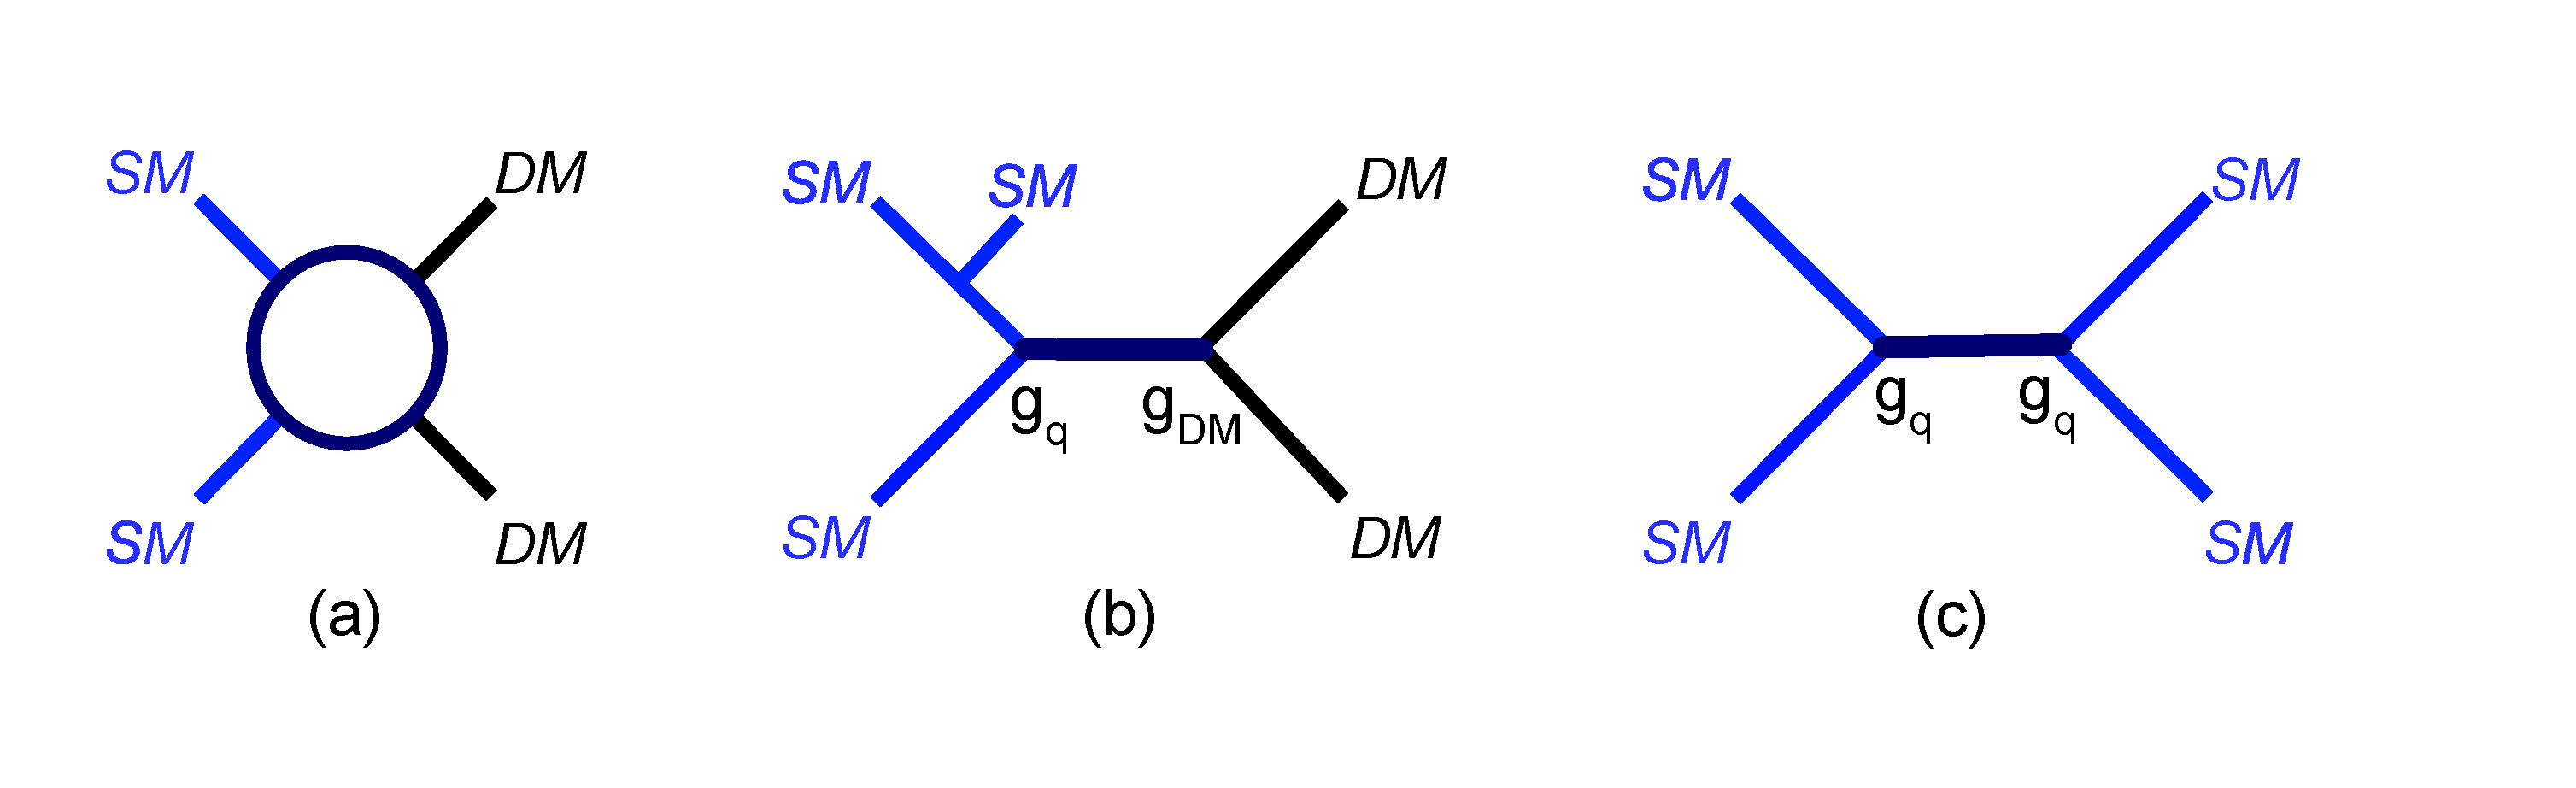
\includegraphics[width=\textwidth]{figures/MonoX.pdf}
\caption{Sketches of (a) the DM--SM interaction in an effective field theory (EFT), (b) a corresponding simplified model mediated by a BSM particle (with additional radiation off one initial state quark) and (c) the same model where the mediator decays back into SM, with coupling constant for the mediator-quark-quark vertex, \gq, and constant for the mediator-DM vertex, \gdm. From~\cite{monoXfig}.}
\label{fig:monoX}
\end{figure}


The standard models include models with neutral mediator particles singly-produced at the LHC and decaying to pairs of \IP, and to pairs of SM particles (Figure~\ref{fig:monoX} (b) and (c)). Two-body mediator decays are simple, attractive benchmarks. Colored mediators allow vertices involving only one DM particle and phenomenology akin to that of SUSY models with a squark mediator~\cite{Papucci:2014iwa,An:2013xka,Bell:2012rg}. 

Models of BSM mediation can be classified according to the spin of the mediator: spin-1 vector or axial vector mediators (\Zprime), scalar mediators (termed $\phi$ in the following) and spin-2 mediators. Spin-2 mediator benchmarks have not yet been adopted by LHC searches; they produce diboson signatures not present in other models~\cite{Kraml:2017atm,Han:2015cty}.

For additional decay signatures, for 'dark sectors' of many additional particles, and for far larger LHC datasets than at present, many more simplified models become interesting. Ref.~\cite{Arcadi:2017kky} provides a review. %[cite co-annihilation codex? other inventories? note that we have already told them about other reviews earlier]



%%%s-channel
\textbf{Massive color-neutral spin-1 bosons with vector or axial-vector couplings} are nearly ubiquitous in BSM theories, so \Zprime as the mediators connect with a wide class of models~\cite{Shoemaker:2011vi}.
Since the \Zprime coupling to quarks must be non-zero for its production at the LHC, both invisible and dijet signatures are discovery channels.
This coupling (or loop-level coupling) to SM partons is also required for nuclear recoils in underground DM searches.
%Parameters
The models in use at ATLAS and CMS contain either vector, axial-vector, or mixed couplings to quarks and a single species of \IP.
The couplings of the \Zprime (\gq to all quarks, \gl to leptons, and \gDM to \IP), the mass of the \IP particle \mdm, and the \Zprime mass \mmed are free parameters.
Lepton decays, if not included explicitly at tree level, arise through the quark coupling at loop level (see Ref.~\cite{Albert:2017onk} and references therein). Decays of the spin-1 mediator into neutrinos are also required by gauge invariance, and add an invisible decay channel that can enhance signatures of missing transverse momentum, depending on the size of the couplings~\cite{Albert:2017onk}. 
The spin structure of the \Zprime couplings does not significantly change the LHC phenomenology, but has a much larger effect in signals in non-collider searches. 
 %leading to a mixing between the Z' and the Z

%%changes the comparison of LHC results to DD and ID searches.
%Axial vector are the most widely used LHC benchmarks as DD rates are suppressed. 

%Additions: Higgs and Z' models
\Zprime mediated models can include additional couplings of the \Zprime to acquire mass through a new baryonic Higgs $h_B$~\cite{Berlin:2014cfa} that collapses to the simpler model above in the limit of very heavy \Zprime mass. 
%When the interaction between the \Zprime and the SM Higgs is relevant, it can be parameterized using the \Zprime-SM Higgs coupling \ghZprimeZprime and the mixing angle between the SM Higgs and the baryonic Higgs, \sinthetab. 
%which in turn is a function of the vacuum expectation value of $h_B$. 
%This model can also lead to mono-Z signals, if the \Zprime is allowed to interact with the Z and the photon through kinetic mixing, 
%but this interaction has so far been neglected in LHC Run-2 searches. 
%CD: is there a paper by Vichi on this topic? Can't find it
They can also be embedded in a Type-II Two-Higgs Doublet Model (2HDM)~\cite{Berlin:2014cfa,Liew:2016oon}.
%, where
%it does not decay directly into DM but instead decays into a new pseudoscalar $A^0$ and
%a SM Higgs boson with a coupling \gZprime~\cite{Berlin:2014cfa,Liew:2016oon}. Here the model parameter
%space is more complex, even when considering the alignment limit (one of the Higgs from the doublets is the SM Higgs).
%This model includes a mixing between the \Zprime and the SM Z boson that is proportional to
%the ratio between the vacuum expectation values of the new Higgs doublets ($tan \beta$). 

%Problems
With certain values of the model parameters, especially low \Zprime mass,
the model can satisfy the relic density constraints~\cite{Chala:2015ama}.
However, if taken in isolation, the model is non-renormalizable, and the axial-vector
model violates perturbative unitarity in certain regions of the off-shell parameter space~\cite{Chala:2015ama,Kahlhoefer:2015bea,Boveia:2016mrp}. 

%%%%%
%%%%%
%%%%%

% If the mediator is a real scalar or a pseudoscalar singlet, it can have tree-level interactions with DM.

\textbf{Color-neutral scalar and pseudoscalar bosons} are an BSM analogue of the Higgs portal model. In comparison to the \Zprime models, a BSM (pseudo-)scalar mediator model~\cite{Buckley:2014fba},  
has some additional peculiarities. 
Under MFV, the couplings of the (pseudo-)scalar bosons to fermions are mass-dependent. As with the Higgs boson, this has three familiar consequences: mediator production through loop-induced couplings to gluons~\cite{Haisch:2015ioa,Mattelaer:2015haa} and associated with heavy flavor quarks~\cite{Buckley:2014fba};
    production cross-sections are smaller than for vector mediators;
    and visible decays of the mediator are dominantly to third generation quarks. 
Despite lower production cross-sections, the more specific experimental signatures allow for these models to be tested during LHC Run-2.
%Single top signatures are also in reach of LHC searches~\cite{Pinna:2017tay}, as they are kinematically favored even though their production cross-section is generally lower with respect to the associated production of a pair of top quarks. %CD: this is interesting and new, but may be cut if we need to cut. 
%Remaining flavor constraints~\cite{Dolan:2014ska}.

%Parameters
The (pseudo-)scalar models used by ATLAS and CMS are fully specified by the masses of the \IP and the mediator, the $\phi$-\IP coupling (\gdm), and the $\phi$-fermion (\gq) coupling.
Following the convention in~\cite{Abercrombie:2015wmb}, \gq is a pre-factor to the Yukawa couplings to fermions and set equal for all quarks.
For the same model parameters, the scalar and pseudo-scalar models predict similar kinematic distributions.
%Since the pseudoscalar model has been favoured for the interpretation of the DAMA and galactic center excess~\cite{Arina:2014yna,Agrawal:2014una} and collider searches are favored when comparing to DD~\cite{Banerjee:2017wxi}, LHC searches have privileged this choice and considered the associated scalar boson as decoupled at higher energies. 

%CD: this needs a feynman diagram otherwise one gets confused
When introducing an additional scalar, one must consider how the scalar relates to the Higgs boson. Large mixing with the Higgs can lead to strong constraints from Higgs measurements. In Ref.~\cite{Berlin:2014cfa}, the scalar can couple to DM through a Higgs portal~\cite{Berlin:2014cfa}. %The coupling between the scalar and the Higgs is $b$ (set to unity for simplicity, and the mixing angle is \sinthetahS, constrained to be below 0.4 by Higgs precision measurements. The values of these two parameters don't affect the kinematics significantly. 
%Where it is applicable and what are the pitfalls
%Maybe add Uli/No/etc's papers here?
If the mediators are pure SM singlets, the model is not invariant under $SU(2)_L$~\cite{Bell:2016ekl}. 
To restore gauge invariance, mixing with the Higgs sector is crucial. 
Couplings to the electroweak gauge bosons can also be added as a consequence of electroweak symmetry breaking~\cite{Bauer:2016gys,Englert:2016joy}. The tree-level signatures in this case include Higgs or vector bosons plus missing transverse momentum and, if the \IP are sufficiently light, invisible decays of the Higgs boson.
%CD: check back on emails with DiFranzo


%%%t-channel, colored
%General
\textbf{Colored scalar and pseudoscalar bosons} allow direct coupling between SM carrying color and \IP carrying $Z_2$ charge~\cite{Bai:2013iqa, Papucci:2014iwa, An:2013xka, Bell:2012rg}. Colored mediators can have a broader set of multi-jet signatures and kinematic features than the neutral mediator models, including the radiation of vector bosons by the mediator~\cite{Bell:2012rg}. 

%Parameters
In colored (pseudo-)scalar models, the mediator must be heavier than the \IP to ensure \IP stability. 
%The mediator mass is set equal for all mediators due to the MFV assumption,
%Requirement of the width: mChi^2+mq^2<=Mmed^2
For the current LHC results, the coupling, \gdmq, between \IP and quarks, the \IP mass, and the mediator mass are free parameters. 
%However, if only right-handed, down-type quarks are considered, flavor constraints do not exclude a significant part of the parameter space~\cite{Abercrombie:2015wmb}. 
%CD: the previous sentence does not have a source, and the Bell model only uses left-handed quarks. This is a question for Millie and the theorists present tomorrow. 

The exchange of a scalar colored under SU(3) is analogous to squarks in the MSSM where only squarks and neutralinos are light.
In the MSSM, the coupling between DM and the squark is constrained to be small\cite{Abercrombie:2015wmb}.
Without the requirements of a SUSY framework, this coupling need not be small. 
For example, if the DM is a standard thermal relic, the couplings required to obtain the correct dark matter density are generally higher than what used by SUSY models.
Models with three generations of mediators can satisfy flavor constraints and the SM gauge symmetry~\cite{Ko:2016zxg}. 
%Citation to MG's studies?
%Couplings to vector bosons also allow the mediator to radiate a W or Z, leading to collider signatures that can be targeted by searches looking for this radiation~\cite{Bell:2012rg}. 

%Problems 
%If one tunes the parameters and couplings of this model to describe gamma ray excess and motivate searches with a single $b-$quark in the final state~\cite{Agrawal:2014una}, leading to a similar phenomenology as the MSSM with a light bottom squark and neutralino. 
%Top-flavored models also exist in literature but have not been used as benchmarks in LHC searches. 

\subsubsection{Less simplified models}
\label{sec:LessSimplifiedModels}

%The initial list of models recommended to the experimental collaboration by the Dark Matter Forum described above is a first set of simple, mostly tree-level processes targeting early Run-2 searches. 

Simplified models can guide the design of generic searches but do not cover the full complexity of possible collider signatures that arise in more complete models.
On the other hand, relying too heavily on a small sample of complete models risks focusing searches too narrowly on an unrepresentative set of signatures.

There are a large number of "less-simplified" models that attempt to find a middle ground between models that are too simplistic and those that are unnecessarily complex. Because the set of such models grows quickly with the number of ingredients, and there is not a broad consensus on which models should be a priority, very few of them have been explicitly considered by LHC searches. Here, we highlight a few such models with different signatures than the simplified models described above. 

\textbf{Co-annihilation} models add two specifies of dark sector particle, one close in mass to the other. Examples can be found in Refs.~\cite{Buschmann:2016hkc,Baker:2015qna,Khoze:2017ixx}. The interaction between these two states drives the cosmological history~\cite{Ellis:1999mm,PlehnLecturesDM}, as processes involving both types of particles can efficiently annihilate into SM particles. The LHC signatures include missing transverse energy and multiple hadronic jets accompanied by multiple resonant or non-resonant hadronic jets, but can be very diverse, encompassing signatures typically found in wildly different BSM models (e.g., searches for lepto-quarks). In some cases, these signatures are untested by any current LHC search~\cite{Buschmann:2016hkc}. 

Most simplified models in use at the LHC assume MFV to ensure that the models are compatible with a vast and unwieldy assortment of experimental constraints on flavor-violating processes. Nevertheless, viable \textbf{non-mimimal flavor-violating models} can be constructed, but one must then understand the impact of the many constraints \cite{Blanke:2017tnb}. Mediators that couple to dark matter and a top quark are one category of flavor-violating model that remains least constrained by low-energy measurements~\cite{DHondt:2015nat}. These yield a distinct 'mono-top' LHC signature. 

Other~\textbf{models with multiple mediators} with small couplings to SM particles have been developed to escape existing LHC constraints~\cite{Duerr:2016tmh}. 

%[add more models that we find interesting if we have time. Other types of initial states, gluphilic, and lepton DM that we can't produce at the LHC but at LEP.]
%Dark terminator needs Majorana particle, not mentioned although the idea of vector + scalar is interesting beyond LianTao's 2HDM
%OOutline said gluphilic, but we cited it above and we need to save space

%JUNK: However, as we will see in Sec.~\ref{sec:LessSimplifiedModels}, this complexity does not translate into significant changes in the LHC kinematics of the simplest models, but rather adds extra signatures for LHC searches. Meaning: it can be rescaled. 

%Problem: we don't know whether scalar sector of the SM is only Higgs or there's a more complex Higgs sector.

The recent discovery of the Higgs boson places LHC at the forefront of the exploration of the SM scalar sector. Ultimately we don't yet know whether this scalar sector is limited to the SM Higgs boson. A single scalar mediator may not encode all important features of the more complicated phenomenology of more \textbf{complex scalar sectors}. Extended scalar sector models often involve signatures with \MET accompanied by the Higgs or other SM bosons.
One step beyond the simple scalar mediator model is to take mixing between this mediator and the SM Higgs boson, dictated by gauge invariance, into account~\cite{Bauer:2016gys,Berlin:2014cfa}. 
A much larger step beyond this is to consider an extended Higgs sector such as a Two-Higgs Doublet Model (2HDM) where one or more of the scalars acts as the SM-DM mediator~\cite{Bauer:2017ota,Ipek:2014gua,No:2015xqa,Goncalves:2016iyg,Bell:2016ekl}. In these models, the new  mediator mixes with the Higgs partners rather than with the SM Higgs, so that the model remains compatible with Higgs measurements. Some models developed for LHC searches focus on one Yukawa structure (Type-II). The particle content includes two CP-even bosons (one of which is the SM Higgs boson), two CP-odd bosons (of which one is the pseudoscalar DM mediator), two charged Higgs bosons, and the \IP. Masses and couplings of these models are chosen to respect vacuum stability~\cite{No:2015xqa}, electroweak and flavour constraints, and to reproduce the observed dark matter abundance.

%Depending on the parameter chosen, this model can satisfy the relic DM density, in general with values of \mdm above 100 GeV.   
%%Overkill?
%[1] M. Bauer, U. Haisch, F. Kahlhoefer, CERN-TH-2017-011, DESY-17-010 [arxiv:1701.07427 [hep-ph]].
%[2] S. Ipek, D. McKeen and A. E. Nelson, Phys. Rev. D 90, no. 5, 055021 (2014) [arXiv:1404.3716 [hep-ph]].
%[3] J. M. No, Phys. Rev. D 93, no. 3, 031701 (2016) [arXiv:1509.01110 [hep-ph]].
%[4] D. Goncalves, P. A. N. Machado and J. M. No, arXiv:1611.04593 [hep-ph].
%[5] N. F. Bell, G. Busoni and I. W. Sanderson, arXiv:1612.03475 [hep-ph].
%^The richer span of experimental signatures permits to expose uncovered regions in the parameter space of the model, as well as to highlight the complementarity between final states. 

%Sam's LianTao's 2HDM checks
%https://docs.google.com/presentation/d/10R9XJaoMDEhXKhd_Wx9yMXEaPl4uXR8IcmuTeLancvg/edit#slide=id.g217998804d_0_47

\subsection{Supersymmetric models and other complete theories}
\label{sec:SUSYModels}

So far, we have considered rather general simplified models inspired by interactions found in the SM. These are obviously far from all the possibilities. %so their combined phenomenology cannot be considered a comprehensive list of the ways in which DM could manifest in a collider experiment.
 Further sources of inspiration for searches are the large number of BSM theories that have been developed to solve theoretical problems of the SM, and the mechanisms through which these provide \IP candidates. 

%AB sentence which I liked better than mine
%Supersymmetry (SUSY), besides solving many theoretical problems of the Standard Model, often provides a dark matter candidate. 
Superymmetry (SUSY) is one class of such theories, postulating partner particles to all SM degrees of freedom to stabilize
the mass of a light Higgs boson.  
Reviews of supersymmetric DM models can be found in \cite{Feng:2010gw,Ellis:2010kf}.
Instead, we will broadly sketch models relevant to
recent experimental progress and stress where we expect future developments. 

Supersymmetric relic dark matter, the archetype for the WIMP idea, has a long
history \cite{doi:10.1016/0550-3213(84)90461-9}. Of these, the most viable and well-studied has been neutralino dark matter. 
The neutralino, a spin 1/2 partner particle to the SM gauge bosons, is often assumed to be the lightest supersymmetric particle (LSP). 
R-parity conservation makes the LSP being stable~\cite{Farrar:1978xj} and prevents proton decay. 
%this is a Frederik-suggestion, not sure I'd put it here as it's implicit
%making it a viable DM candidate as it is weakly interacting, neutral, massive and stable.  

%, a key feature of many SUSY theories 
%featuring supersymmetric partners of SM particles. 
%maybe we could cut, but we need it if we want to mention that make clear that gravitino needs to be RPV to be observed
In the Minimal Supersymmetric extension of the Standard Model (MSSM),
%, where superpartners have the same mass as their SM counterparts
%this could be a sidebar where one explains that SUSY needs to be broken to have masses that are not SM
there are four neutralinos, each a mixture of SM boson superpartners: a wino, a bino, and two higgsino fermion states.
The lightest neutralino may be called 'bino-like,' 'wino-like,' or 'higgsino-like'
in regions of MSSM parameter space where one of these components dominates the mixture.
The phenomenology of these  is different from most of the simplified models in the previous section, and it depends on mixture and on the particle spectrum. 
The LHC signatures feature missing transverse momentum from the neutralino and a high multiplicity of other objects
(leptons, jets) produced in cascade decays of heavier superpartners.  
%Sufficiently energetic cascade products can serve as additional experimental handles,
%allowing specially-optimized searches to target specific benchmark models with potentially far better sensitivity than a generic search. 

%JUNK: If the next-to-lightest SUSY particle (NLSP) is much heavier than the LSP, the LSP will be boosted and produce
%a large amount of missing transverse momentum. If instead the mass spacing between NLSP and LSP is 
%small (compressed scenario) there will be only room for a limited amount of \MET in the event.

%FR: (I can't stress this point enough, the number of actual extra/BSM degrees of freedom can be as low as 5, one only ends up with 100+ parameters when not knowing or not making any assumptions on the GUT scale physics and mechanism to break SUSY)

%FR: Here you go. Mainly small comments, the only sort of major one being
%@MSSM. Its in the document also, but just to clarify, its a framework
%or class of theories/models built bottom up. Take the minimal particle
%content, try to  classify the phenomenology, but largely ignore what
%really happens e.g. at the GUT scale or how SUSY is broken.
%
%Hence:
%1. I wouldnt call it complete theory, its not. mSUGRA is a complete
%theory for example
%2. We perfectly well know SUSY does not have 100+ independent
%parameters, due to constraints from flavour physics, ... . It might be
%as low as 5 (mSUGRA), but in the context of the MSSM we dont know the
%minimal set of eigenvectors to span the space, the correlations and so
%on (as we dont know how and why SUSY is broken), so we have 100 "free"
%parameters, but just in ignorance of what the real eigenset is.
%Breaking that down to 20ish is not really just to simplify, but is
%"just" assuming a certain set of independent eigenvectors.

The MSSM is a complete theory with more than 100 independent parameters, 
but realistic SUSY models might be far simpler.%reduced to far fewer independent degrees of freedom using experimental knowledge and theoretical assumptions (e.g. universality of certain particle masses or parameters). 
Such models are used as predictive benchmarks for DM searches. 
One of these is the phenomenological MSSM (pMSSM), which assumes no sources of CP violation beyond the SM nor Flavour-Changing Neutral Currents, and retains universal couplings and masses for first and second generation superpartners, reducing
the number of MSSM parameters to 19. 

Another DM candidate in gauge- or gravity-mediated supersymmetric models is the gravitino, 
%MSUGRA: gravitino is too weakly interacting? unclear
a 3/2-spin particle superpartner of the graviton. 
Gravitino interactions are suppressed by the Planck scale (10$^{18}$ GeV) before SUSY breaking.
%the caveat is that some stuff happens during SUSY breaking and improves the rates, but 10^18 is a shitton
This has consequences both on their viability as a thermal relic and on their phenomenology. 
In gauge-mediated SUSY, the gravitino can be a DM candidate for a
non-standard cosmological history~\cite{Steffen:2007sp}. 
%For AB: I am not sure this is enough...
%and a mass below the GeV~\cite{}. 
%https://arxiv.org/pdf/hep-ph/9801417.pdf
%While very light gravitinos (eV masses)
%will not contribute significantly to the total mass density of the universe, if
%the gravitino LSP is too heavy (m g >? few keV) its relic mass density in 3/2
Similar to the neutralino case, the identity and masses of heavier states decaying to the gravitino LSP determine its phenomenology. However, the gravitino interactions are very weak, posing problems for 
direct and indirect detection searches. 
%In this case, searches need to exploit
%particular features of the signal, as described in the next section. 
%Frederik thinks the logic here is not too clear, I would agree
%What he says: make it clearer that observation with an inclusive selection is difficult
%but isn't that too experimental for this section? We only need some link to the
%LLP part below. Yes.
%Observation at colliders is difficult using inclusive selections due to the low rates of direct production,
%but additional experimental features from the long-lifetime of coannihilating long-lived NLSPs
%can be used to discriminate between rare signals and backgrounds. 
%here and above we are specifically thinking of tau because it gives a good relic, maybe worth mentioning later

%Even though the gravitino does not easily constitute a good
%thermal relic candidate, it provides different signatures 
%i found Bolz:2000fu that says it's a good one

Because of the huge variety of potential experimental signatures, SUSY searches also often adopt a simplified model approach, 
decoupling the particles that determine the lowest energy collider phenomenology
(generally LSP and NLSP) from the rest of a heavier particle spectrum~\cite{Alves:2011wf}. 
As in the general simplified models described earlier, extending the MSSM quickly generates a plethora of non-minimal possibilities.
%Examples are models where a right-handed neutrino is added to the SM leading to a SUSY DM candidate with signatures privileging leptons~\cite{Arina:2015uea},%this motivates monoW
%and R-parity violating models, 
%or models that add to the minimal particle spectrum of the MSSM superpartners. 
%if you think this is too vague, we kill it

\subsection{Long-lived particle models}
\label{sec:LLPModels}

%Connection to SUSY

Another class of models found within and beyond SUSY are models feature suppressed cascade decays of a heavier particle (the NLSP in SUSY) to a lighter particle (the DM LSP in SUSY). The suppression can be so large that the particle travels a macroscopic length within the detector before it decays. Within SUSY, one way to achieve this suppression is for the NLSP to decay through a heavy intermediary. Split supersymmetry models are a subset of SUSY models where the gluino must decay through a heavy, off-shell squark~\cite{Masiero:2004ft}. The heavier the mass of the squark, the longer-lived the gluino. %This is akin to the W-mediated decay of the pion. 
Alternatively, the NLSP decay can be heavily suppressed by some power of the mass difference with the LSP. This mass difference also affects DM co-annihilation rates and therefore the DM abundance~\cite{Ellis:1999mm}.
Finally, another way to achieve long-lived decays is with parameterically small couplings, as in the case of gauge-mediated supersymmetry models where the long-lived NLSP decays to its SM partner plus the gravitino~\cite{Dimopoulos:1996vz}, with a SM analogue in the Cabibbo-suppressed B-meson decays.
Because of the prevalence of these mechanisms, it is important to look for long-lived cascade decays.

Besides SUSY, one can find long-lived signatures within the generic simplified models in Sec. \ref{sub:simplifiedModels} for small enough couplings. If one assumes thermal freeze out, the coupling of the mediator to DM pairs is bounded from below to obtain a sufficiently large annihilation cross section. However, it's anybody's guess what mechanism in the early universe was responsible for the observed DM density. In alternate scenarios, such as "dark freeze out" where DM can annihilate directly to BSM mediators but not viceversa, the mediator couplings to the SM can be far smaller than allowed in standard thermal freeze out~\cite{Pospelov:2007mp,Das:2010ts}. The couplings of the mediator therefore can be small enough that it is long-lived. Despite such small couplings, a sufficiently light mediator can be produced at colliders with appreciable cross section. Many models have been proposed in this direction. For example, DM can interact with the SM via a dark vector boson of a U(1)' dark symmetry, equivalent to the SM's U(1) but with much smaller couplings~\cite{Holdom:1985ag}, such as those originated by kinetic mixing. The freeze-in scenario~\cite{Co:2015pka,Bernal:2017kxu} is another possible for very weak DM--SM interactions such as those of dark photons.

The mediator can also be a dark scalar boson (a "dark Higgs") that only couples to the SM, akin to a Higgs portal~\cite{Curtin:2014cca}. 
[add sentence about coupling with the higgs by Curtin and exotic decays of Higgs boson]
%or via mixing with a heavy pseudoscalar in 2HDM with a coupling $k$. Who cares, maybe also who cares about the mixing even. 
%The reason why it is interesting is because ID is suppressed but it's also very hard to discover at colliders.
In both cases, the dark boson mediator can be light and long-lived~\cite{Pospelov:2007mp}, and its visible decays into SM particles or associated production with a SM boson provide the main collider handle for observation~\cite{Curtin:2014cca}.
These scenarios can also be probed by complementary beam dump and fixed target experiments~\cite{Battaglieri:2017aum}. %maybe in results section?
Simplified co-annihilation models with long-lived particles have also been proposed~\cite{ElHedri:2017nny}. 
%, including present and future colliders, as this model includes decays of the dark boson into SM fermions as well as into DM particle, and include Higgs decays. 
%Z width, contact interactions
%Relic connection
%There is still a large possible dark boson and DM candidate mass range that is still compatible with thermal freeze-out~\cite{Das:2010ts}. 
%Further examples of the third case can be connected to the simplified models described in Sec.~\ref{sub:simplifiedModels}. If the only connection between the DM and SM is the new mediator particle, and e.g. when DM can annihilate directly to BSM mediators and not viceversa (as \mdm $>$ \mmed), then the couplings of the mediator to the SM can be arbitrarily small.

%To illustrate this mechanism, in Section 2 we will construct several models with fermionic, scalar and vector particles as mediators. We show that if mWIMP < mmediator, the parameter space of such models is highly constrained, as the coupling of the mediator to the SM must necessarily be sizable to ensure the required annihilation cross-section. Yet if the reverse is true, mWIMP > mediator, there are no strict requirements on the size of the mixing except for the lifetime of the mediator state, which in some instances can be satisfied for (mixing)2 of the mediator with the SM as low as 10−23.

%when the couplings between the partner particle and either SM or DM particles are small, as in the SM example of the Cabibbo-suppressed B-meson decays, or in the example of 
%produced with appreciable cross-sections at the LHC. 

%If the mass difference is lower than 100 MeV, the NLSP may be long-lived as the available phase space
%for its decay into LSP and SM particles is limited, %this is a repetition but if I were a student I would like to know why
%leading to signatures of long-lived particles~\cite{Chen:1995yu}. 

%MET in the limit of long-lived
%As discussed in the introduction to this chapter, the LHC does not directly detect DM, but rather uses visible objects to signal the presence of non-interacting, long-lived particles that escape detection. If the particle does not decay, then it is a good DM candidate. In many non-WIMP, dark sector models, one can postulate the existence of DM particles as well as other particles with lifetimes not long enough to be cosmologically stable~\cite{Strassler:2006im}. Those particles escape conventional detection by collider experiments, as they e.g. decay half-way through the detector.
% and may lead to signatures of missing transverse momentum.
%this is ambiguous: they can also lead to MET if they decay invisibly?
%However, these dark sector particles usually do not carry sufficient energy to be observed by traditional searches, so experiments must devise methods that specifically target those non-standard decays. These will be discussed in Chapter~\cite{sec:03_ExperimentalResults}.
%JUNK: The small mass splitting between the two particles forces the decay of the next-to-lightest particle into the lightest particle to be kinematically suppressed, in turn leading to a sizable lifetime for the next-to-lightest particle~\cite{Khoze:2017ixx}. The late decays of the coannihilation partner give an additional experimental handle that can be used for LHC searches, as described in the next chapter.  

\subsection{Dark interactions}
\label{sec:darkint}

%this sounds like the conclusions of the whole paper not the conclusion of this chapter
In the above, we've sketched some of the models and signatures that are currently being sought at colliders. Next, we review experimental searches for invisible particles, in light of the models discussed above. Nevertheless, we have left many models uncovered. From one point of view, any model containing stable particles interacting feebly with the SM is a theory of DM. Drawing the connections between this model and astrophysical DM is challenging, but this is the key difference between models of DM and other models of BSM physics. 

%One might think of DM theories as classes of models postulating a new "dark sector" that has only feeble connections with the SM, or is secluded from it. 
The dark sector can be arbitrarily complex, as long as the particles and interactions it contains satisfy cosmological observations~\cite{Strassler:2006im}. The models listed above are simple examples of such dark sectors, where the mediator particles (e.g. dark bosons) provide the connection with the SM. Many other models are worthy of mention here, including asymmetric DM models, where dark sector particles and antiparticles are not produced in equal amount, in the same fashion as matter and antimatter for SM baryons~\cite{Zurek:2013wia}, and models of "neutral naturalness" realizing a mirror copy of the SM without any low-mass equivalent of the SUSY colored partners~\cite{Craig:2014aea}. 
% . that evade the experimental constraints described in the next chapter
%minimal DM: https://arxiv.org/pdf/hep-ph/0512090.pdf
%dynamical DM: https://arxiv.org/abs/1106.4546
%dark QCD & emerging jets: https://arxiv.org/abs/1306.4676 https://arxiv.org/abs/1502.05409 could link to asymmetric DM

%Other orphan models
%Other BSM theories including DM particle candidates that are not covered in this review are
%extra dimensions~\cite{Hooper:2007qk}, and sterile neutrinos as DM~\cite{Adhikari:2016bei}.
%If we want to summarize we can look here: http://www.slac.stanford.edu/econf/C040802/papers/L002.PDF
%For AB who has book: See Bertone's book for other non-SUSY candidates at the EW scale? 
%\cite{FengAR} %x-devonthink-item://F9E6F4B6-265D-48CF-B8CC-48B17D28C0DC

%Previous text
%but also give up some of SUSY's desirable features. 
%An example is neutral naturalness, a theoretical framework that features a mirror copy of the SM,
%with no equivalent of the SUSY colored partners whose mass scales have been
%pushed beyond the "natural" TeV scale. Models realizing "neutral naturalness"
%include dark sector particles with non-standard signatures and Dark Matter candidates similar to the
%Asymmetric Dark Matter models mentioned above~\cite{Garcia:2015toa},
%and it will be testable at colliders beyond the LHC. 

%dynamical dark matter?

% a secluded



%goal of this section:

%- explain dark sectors / hidden valleys / dark photon connection and relevance
%- highlight neutral naturalness and asymmetric dm


%riefly mentioning a few ideas that [are important to the future / we think are cool or important / we haven't explored but should].







%Nevertheless, there are many uncovered
%ideas leading to new collider paradigms for DM beyond the basic models described so far. Looking for the connection
%between the SM and DM is equivalent to looking for new feeble interactions, a topic with which much of the collider
%program is engaged and that will continue evolving in both theoretical and experimental directions. Many 
%ideas achieve a so-called "dark sector" 

%[has a long way to go and we started with the most basic searches]

%has only started with the design of most basic searches, and there are plenty of 

%'ve only [scratched the surface] and there are plenty of ideas we haven't covered. [There is a big wide world of dark shit.] In a sense, looking for connection between SM and %DM is looking for new feeble interactions, a topic with which much of the collider program is engaged. There are many ideas to acheive a so-called 'dark sector', i.e. a new, %hidden BSM sector of matter that interacts with the SM through [only a few special portals or mediators or whatever].

%hidden valleys, asymmetric dm, neutral naturalness, grab bag of other stuff.

%The absence of SUSY signals in the first LHC data, as detailed in Sec.~\ref{03_ExperimentalResults}
%has also generated interest in theories that can evade those constraints. 

%Aside from dark matter comprised of neutralinos, DM could be consistuted from gravitinos. Gravitino DM would not be a thermal relic (because only gravitational strength interactions, cite?). At colliders, it could be produced by the decay of heavier SUSY states. Similar to the neutralino cases, the identity and mass of the heavier states (i.e. the NLSP) determine the signatures, but for the gravitino the favored signatures are different. 
%- NLSP could be stop i.e. tops + MET signature
%- NLSP could be stau, metastable charged particle at the LHC, relatively long-lived (non-prompt) lepton signatures
%- NLSP could be sneutrino and so forth.



